\documentclass{article}

\usepackage[utf8]{inputenc}
\usepackage[T1]{fontenc}
\usepackage{lipsum}
\usepackage{graphicx}
\usepackage{amsmath}
\usepackage[margin=1in]{geometry}
\usepackage{titlesec}
\usepackage{enumitem}

\titleformat{\section}
{\LARGE\bfseries}{\thesection}{1em}{}

\titleformat{\subsection}
{\Large\bfseries}{\thesection}{1em}{}

\begin{document}

\pagestyle{empty}


\section*{HW4}
\large

\subsection*{Traccia}
\large
Una macchina distributrice di cibo e bevande accetta pagamento in monete, eventualmente fornendo il resto, oppure tramite una chiavetta prepagata. Si tracci un diagramma di stato UML che descriva il comportamento atteso della macchina. Si tracci poi un ulteriore diagramma di stato UML che realizzi il comportamento atteso richiamando le opportune operazioni definite nella classe \textit{VendingMachine}. All'interno della seconda macchina i comportamenti possono essere definiti come azioni associate alle transizioni o come azioni enter/do/exit associate agli stati. 

\subsubsection*{Risoluzione}
Per poter rappresentare al meglio uno state diagram è bene porsi nei panni della realtà che dovrà essere modellata, data che non potranno essere illustrate attività ma solo condizioni a cui sottostare, si ricordi che la descrizione degli stati avviene tramite l'utilizzo di partecipi al loro interno. In relazione al primo \textit{chart} potrebbero essere adeguati differenti flussi di esecuzione, i quali a loro volta tendono ad aumentare la complessità modellativa; si potrebbe porre come primo stato la \textit{selezione del prodotto}, l'\textit{immissione di monete} oppure la combinazione delle due. Si osserva come l'ultima scelta introdotta rappresenti un livello di difficoltà maggiore delle prime, in cui occorre stabilire una transizione che renda accomunabili i due processi esecutivi di selezione e acquisto del prodotto.\vspace*{14pt}\\
Nonostante di seguito è introdotto un diagramma che pone un certo flusso di esecuzione, ovviando alla possibilità di dinamicità alla realtà di una macchina distributrice.

\subsubsection*{Primo UML state machine diagram}
\large

\textit{Diagramma errato}
\begin{center}

\includegraphics[width=1\textwidth]{foto 6.png}    
\end{center}

\subsubsection*{Considerazioni}
Il diagramma pone un livello di complessità più elevato del necessario, tuttavia alcuni elementi per la realtà modellata sono introdotti correttamente. Innanzitutto è giusto stabilire una transizione ciclica che richieda l'inserimento di altre monete fino a quando non si raggiunga il credito necessario, ciò si potrebbe adeguare anche per la fase di \textit{selezione}, in cui il token è mantenuto nello stesso stato affinchè non sia posto uno \textit{string matching} adeguato rispetto ai codici univoci dei prodotti contenuti.\vspace*{14pt}\\
Nonostante, gli elementi negativi sono di numero maggiore e più importanti. L'aumento della complessità è data dalla presenza dello \textit{pseudostato fork}; un fork allude alla presenza di due nodi iniziali di esecuzione che corrispondano a processi esecutivi paralleli, per cui in questo caso, è sbagliato considerarli come due flussi differenti. Per cui è bene eliminare lo pseudostato introducendo due percorsi contraddistinti, i quali successivamente si uniranno ad un nodo decisionale che comprenda l'insieme di archi uscenti per concludere nello \textit{stato finale}. Inoltre, è errato porre al di sopra del fork eventi e azioni, essi devono essere totalmente liberi da vincoli.\vspace*{14pt}\\
Concludendo, un'ultima nota considera la necessità di un \textit{evento} posto tra lo stato che precede il fork e la transizione che termina nello pseudostato; un evento è valutato più di una volta, differentemente dalla guardia messa a disposizione, per cui se non rispettate, i \textit{marcatori} sarebbero costretti a restare all'interno del participio \textit{waiting payment}. Da quanto detto, si evince una regola fondamentale all'interno dei \textit{state machine diagram}, una \textit{guardia} non è mai rivalutata in assenza di transizioni cicliche.\vspace*{14pt}\\
\textit{Diagramma corretto}
\begin{center}
    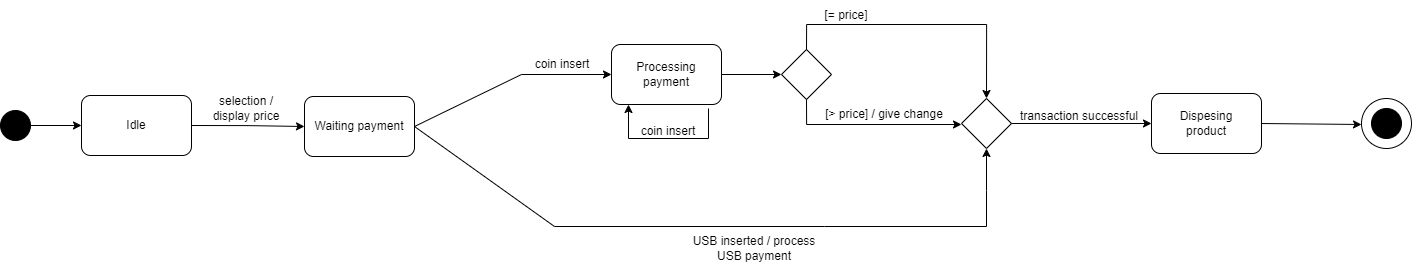
\includegraphics[width=1\textwidth]{foto 7.png}
\end{center}
Nota: il professore non gradisce l'uso delle \textit{choice}, sarebbe bene togliere il \textit{choice} e indirizzare tutte le transizioni verso \textit{dispensing product}.
\subsubsection*{Secondo UML state machine diagram}
\large
\begin{center}
    
\includegraphics[width=0.32\textwidth]{foto 8.png}    
\end{center}
\end{document}